%=====================================================================
%  IEEE AI for Science Congress 2026 / IEEE SocialCom 2026 submission
%  Converted from the ACL-format manuscript "RA-SCOPE"
%  Format: IEEE Computer Society Proceedings (two-column, US Letter)
%  Compile: pdflatex main && bibtex main && pdflatex main && pdflatex main
%=====================================================================
\documentclass[conference]{IEEEtran}
\IEEEoverridecommandlockouts

\usepackage{cite}
\usepackage{amsmath,amssymb,amsfonts}
\usepackage{graphicx}
\usepackage[scaled=0.94]{helvet}
\usepackage{tikz}
\usetikzlibrary{shapes.geometric,positioning,arrows.meta,decorations.pathreplacing,calc}

% palette shared by the TikZ figure and the vector plots
\definecolor{NAVY}{HTML}{1F3B57}
\definecolor{INK}{HTML}{1A1A1A}
\definecolor{OK}{HTML}{12695F}
\definecolor{WARN}{HTML}{C2703A}
\definecolor{BORDER}{HTML}{A9B4BC}
\definecolor{LINE}{HTML}{5A6B78}
\definecolor{PANELB}{HTML}{DCE3E8}
\definecolor{PANELF}{HTML}{F7F9FA}
\usepackage{textcomp}
\usepackage{xcolor}
\usepackage{booktabs}
\usepackage{array}
\usepackage{url}
\usepackage[hidelinks]{hyperref}

\graphicspath{{figs/}}

% tight numeric columns for the results table
\newcolumntype{N}[1]{>{\centering\arraybackslash}p{#1}}

\begin{document}

\title{RA-SCOPE: An Auditable Zero-Parameter Ensemble for Ordinal
Difficulty Assessment of Second-Language Chinese Graded Readers}

\author{
\IEEEauthorblockN{Tingrui You\textsuperscript{1}, Na Zhang\textsuperscript{2},
Ling Xiong\textsuperscript{2}, and Jimei Li\textsuperscript{2,*}}
\IEEEauthorblockA{\textsuperscript{1}Hainan International College, China\\
\textsuperscript{2}School of Information Science, Beijing Language and Culture
University, Beijing, China\\
Emails: yyt2006@163.com; zn17333099816@163.com; lingdonghua99@163.com;
Ljm@blcu.edu.cn\\
\textsuperscript{*}Corresponding author}
}

\maketitle

\begin{abstract}
Assessing the difficulty level of second-language (L2) reading materials is a
recurring educational-measurement task that currently depends on costly expert
panels and produces results that are fragile across publishing platforms. We
present RA-SCOPE, an auditable inference layer for ordinal, book-level
difficulty assessment of L2 Chinese graded picturebooks. Four heterogeneous
monotone experts---length, character n-gram, Standard-derived measurements, and
a fine-tuned Chinese MacBERT---are combined by an unweighted probability pool
that introduces no trainable fusion parameters. A label-free source-distance
support rank licenses a closed-form Euclidean projection of the pooled logits
onto a retained-margin ordinal set, applied only when two complementary anchors
agree and at least one of them is backed by source evidence. Every item
therefore carries an explicit state---CONSENSUS, CONFLICT, or NO-SUPPORT---that
a human review workflow can act on, and every activated consensus grade is
preserved by construction. On 120 independently triple-annotated and adjudicated
Chinese picturebooks, RA-SCOPE reaches .823 quadratic weighted kappa and .417
MAE, improving on fine-tuned MacBERT by .060 and on a Qwen2.5-3B rubric baseline
by .285 (paired 95\% intervals exclude zero), and halving the rate of errors
exceeding one level. A separately adjudicated 28-book collection reproduces the
ordering with no error above one level, and counter-length analyses show that
the gains are not a length artifact. A stacked logistic fusion fitted on
target-collection labels reaches .844 QWK and .275 MAE under cross-validation,
trading the zero-parameter property and the preservation guarantee for lower
absolute error.
\end{abstract}

\begin{IEEEkeywords}
educational measurement, ordinal regression, ensemble inference, readability
assessment, auditable machine learning, human-in-the-loop review
\end{IEEEkeywords}

%=====================================================================
\section{Introduction}
%=====================================================================

Placing a graded reader at the right level is a routine but consequential
educational-measurement decision. Publishers, reading programmes and
curriculum teams must decide whether a book belongs at level~1 or level~4, and
the decision is made under a published standard---the Chinese Graded Readers
Standards for International Chinese Language Education~\cite{cllc2024standards}---rather
than by preference.
Today it is made by expert panels: the collections used in this study were
graded by three annotators with International Chinese Education training who
each contributed approximately 20~hours, followed by adjudication by a fourth.
The cost of that process does not scale with catalogue growth, and its output
is fragile across sources---books that look comparable in length are graded
differently by different publishers because layout, illustration and annotation
conventions differ sharply.

Automatic alternatives are available, but average fit is not what a review
workflow needs. A fine-tuned Chinese encoder reaches .763 quadratic weighted
kappa (QWK) on our main collection, and a deterministic Qwen2.5-3B rubric
prompt reaches only .538 while showing strong sensitivity to surface length.
More importantly, neither returns a decision that a reviewer can inspect: when
such a model changes a grade, nothing in its output says whether the change is
supported by evidence resembling the source material or whether it is an
extrapolation.

Ensembles of ordinal experts make the situation sharper rather than simpler.
Pooling heterogeneous ordinal predictors is known to help, and projection
methods repair order violations, but the literature does not specify which
evidence-backed ordinal decisions a heterogeneous ensemble is permitted to
overturn. That question---not the pooling arithmetic---is what determines
whether an automated grade can be adopted in practice.

We address it with RA-SCOPE (Reliability-Anchored Support-Backed Consensus
Ordinal Projection Ensemble). Four experts first form a monotone probability
pool. Length and character n-gram experts act as complementary anchors, and
source-only nearest-neighbour distances become finite-sample support ranks. A
projection is licensed only when both anchors predict the same grade and at
least one of them has sufficient support. It is the unique Euclidean projection
of the pooled logits onto a retained-margin ordinal set, with a closed-form
solution and no fitted fusion parameters. Fig.~\ref{fig:dataflow} summarises the
design.

Our contributions are:
\begin{itemize}
\item a lineage-disjoint, multi-source evaluation protocol with independent
triple annotation, separate adjudication of every disagreement, a held-out
robustness collection, source-only out-of-fold results, and paired
lineage-bootstrap intervals;
\item a support-backed full-consensus activation rule that never promotes a
single supported anchor to a multi-anchor consensus;
\item a closed-form constrained projection with proofs of monotonicity,
uniqueness, and activated-grade preservation; and
\item analyses of support states, hyperparameter sensitivity, length residuals,
counter-length pairs, Standard-derived construct alignment, and
observable-modality routing.
\end{itemize}

RA-SCOPE is an inference layer rather than a replacement model. It consumes the
cumulative probability chains that the four experts already emit, introduces no
trainable fusion parameters, and returns for each book an ordinal distribution
together with one of three states. That output is what allows the system to be
placed in front of, or behind, an existing human review queue: Section~\ref{sec:deploy}
sets out the resulting triage behaviour and its measured cost.

%=====================================================================
\section{Related Work}
%=====================================================================

\subsection{Readability and Ordinal Modelling}
Automatic readability assessment has moved from lexical, syntactic, discourse
and psycholinguistic measurements~\cite{xia2016text,deutsch2020linguistic} to
hybrid models that combine pretrained encoders with handcrafted
features~\cite{lee2021pushing,zeng2023promptara,zeng2024interpretara,zeng2025self}.
Ordinal objectives exploit label order~\cite{zeng2022enhancing,lim2024improving},
and cumulative rank models enforce ordered
thresholds~\cite{cao2020rank}. Chinese work includes Standard-derived feature
quantification~\cite{li2025quantification}, adaptive pretraining with feature
fusion~\cite{yang2025chinese}, and book-level long-text
modelling~\cite{li2024going}. We focus on inference-time composition and
decision guarantees rather than on another encoder objective.

\subsection{Ordinal Ensembles and Projection}
Projection-based ordinal ensembles decompose learning into ordered
classification hypotheses~\cite{perezortiz2014projection}, and isotonic
projection repairs threshold order~\cite{barlow1972statistical}. In contrast,
RA-SCOPE projects an already-monotone heterogeneous pool at inference time onto
an item-specific feasible set derived from anchor agreement and retained
margins. The constraint therefore governs decision compatibility, not merely
rank consistency.

\subsection{Support and Selective Prediction}
Distance in a pretrained representation space is a strong non-parametric signal
for distributional support~\cite{sun2022out}, and conformal ranks convert
arbitrary nonconformity scores into marginally valid $p$-values under
exchangeability~\cite{bates2023testing}. Calibration and selective prediction
address uncertainty or abstention~\cite{guo2017calibration,ovadia2019trust,
geifman2019selectivenet,xin2021art}; RA-SCOPE instead always returns an ordinal
distribution while exposing CONSENSUS, CONFLICT and NO-SUPPORT states.

%=====================================================================
\section{Task and Evidence}
%=====================================================================

\subsection{Book-Level Task}
For book $i$ the primary target is $y_i \in \{1,\dots,6\}$. Ten secondary
criteria operationalise the Standard: character, vocabulary,
grammar/sentence, discourse, semantic-content, character/plot, genre/theme,
illustration independence, pinyin/annotation reduction, and layout density. The
first seven describe linguistic or content demand; the final three describe
access and presentation. Proficiency inventories follow GF
0025--2021~\cite{moe2021standards}. Each annotation records a best level, a
plausible interval, and evidence pages where needed.

\subsection{Books, Independence, and Adjudication}
Books come from StoryWeaver~\cite{pratham2026storyweaver}, the Global African
Storybook Project~\cite{gasp2026repository}, and the Global Digital
Library~\cite{gdl2026api}. Original-work lineages were audited before analysis;
no book or lineage crosses the source-development and evaluation collections
(Table~\ref{tab:collections}). Annotators P01--P03 independently annotated
randomised spreadsheets; P04 then adjudicated disagreements and checked the
original sources, and is excluded from inter-rater reliability. All four had
International Chinese Education training and each contributed approximately
20~hours. On the 120-book main collection, ordinal Krippendorff's
$\alpha$~\cite{hayes2007answering} is .677 (book-bootstrap 95\% CI [.594,.740])
for global grades and .586 [.524,.638] over 1{,}200 criterion units. Adjudicated
global counts for L1--L6 are 11/35/40/30/4/0. The 28-book robustness collection
is 7/15/4/2/0/0, and its adjudicated global labels equal the three-rater medians
for every book.

\begin{table}[t]
\caption{Lineage-Disjoint Evidence Collections}
\label{tab:collections}
\centering
\footnotesize
\begin{tabular}{lrl}
\toprule
Collection & $n$ & Role \\
\midrule
Source development & 96 & Expert fitting; support calibration \\
Main & 120 & Adjudicated evaluation \\
Robustness & 28 & Separate adjudicated evaluation \\
Upper-band & 51 & Unscored support audit \\
\bottomrule
\end{tabular}
\end{table}

%=====================================================================
\section{Support-Backed Consensus Projection}
%=====================================================================

Let threshold $k \in \{2,\dots,6\}$ denote $P(Y_i \ge k)$. Expert $e$ emits a
cumulative chain $p_{ik}^{e}$, projected with PAVA so that
$p_{i2}^{e} \ge \dots \ge p_{i6}^{e}$. Its point grade is
\begin{equation}
g_i^{e} = 1 + \sum_{k=2}^{6} \mathbb{1}\!\left[\,p_{ik}^{e} \ge .5\,\right].
\end{equation}

\subsection{Complementary Monotone Experts}
The four experts are: (1)~a log-character-count ordinal model; (2)~character
TF--IDF with 2--5-grams~\cite{salton1988term}; (3)~an ordinal model over 16
Standard-derived measurements, including lexical inventories, sentence and page
density, dialogue, and diversity; and (4)~page-pooled Chinese
MacBERT~\cite{cui2020revisiting} with a cumulative ordinal head. Five-fold
lineage-grouped, source-only cross-validation selects hyperparameters. MacBERT
uses three complete seeds, three epochs, and four sampled pages per book and
epoch. The uniform pool is
\begin{equation}
\bar{p}_{ik} = \frac{1}{4}\sum_{e=1}^{4} p_{ik}^{e},
\label{eq:pool}
\end{equation}
which introduces no trainable fusion parameters.

\subsection{Label-Free Support Rank}
Length (L) and character TF--IDF (C) are the anchors, $\mathcal{A}=\{L,C\}$. For
each anchor, lineage-held-out source episodes yield nearest-neighbour
representation distances $d_j^{e}$, $j=1,\dots,M$. For a new item,
\begin{equation}
u_i^{e} = \frac{\sum_{j=1}^{M} \mathbb{1}\!\left[d_j^{e} \le d_i^{e}\right]}{M+1},
\qquad s_i^{e} = 1 - u_i^{e}.
\end{equation}
A large $u$ indicates a source-distance tail; $s$ is its support rank. We mark
anchor $e$ as support-eligible when $u_i^{e} \le .70$ (equivalently
$s_i^{e} \ge .30$). With continuous distances, $s$ is the usual conformal rank
$p$-value; under exchangeability it is marginally
super-uniform~\cite{bates2023testing}. This conditional result licenses a
support diagnostic, not a correctness probability. The projection activates
exactly when
\begin{equation}
a_i = \mathbb{1}\!\left[\, g_i^{L} = g_i^{C} \ \wedge \
\max_{e \in \mathcal{A}} s_i^{e} \ge .30 \right].
\end{equation}
Thus agreement always concerns both anchors; one supported anchor cannot create
consensus. If supported anchors exist but $g_i^{L} \ne g_i^{C}$, the state is
CONFLICT; if neither qualifies, it is NO-SUPPORT.

\subsection{A Closed-Form Projection}
Let $z_{ik}^{e} = \operatorname{logit}(p_{ik}^{e})$ and
$\bar{z}_{ik} = \operatorname{logit}(\bar{p}_{ik})$, with clipping only at the
logit boundary. For an active item, write the shared grade as $g_i^{\star}$ and
retain fraction $\lambda = .5$. Define the convex feasible set
\begin{equation}
\mathcal{C}_i = \Big\{ z : z_2 \ge \dots \ge z_6, \
z_k \ge \lambda \max_{e \in \mathcal{A}} z_{ik}^{e}\ (k \le g_i^{\star}), \
z_k \le \lambda \min_{e \in \mathcal{A}} z_{ik}^{e}\ (k > g_i^{\star}) \Big\}.
\end{equation}
RA-SCOPE returns
\begin{equation}
z_i^{\star} = \operatorname*{arg\,min}_{z \in \mathcal{C}_i}
\tfrac{1}{2}\lVert z - \bar{z}_i \rVert_2^2,
\label{eq:proj}
\end{equation}
and otherwise returns $\bar{z}_i$. The solution is coordinate-wise clipping:
\begin{equation}
z_{ik}^{\star} =
\begin{cases}
\max\!\left(\bar{z}_{ik},\, \lambda \max_{e} z_{ik}^{e}\right), & k \le g_i^{\star},\\[2pt]
\min\!\left(\bar{z}_{ik},\, \lambda \min_{e} z_{ik}^{e}\right), & k > g_i^{\star}.
\end{cases}
\label{eq:clip}
\end{equation}

\noindent\textbf{Proposition 1 (valid ordinal output).} \emph{The pool in
(\ref{eq:pool}) and the projected probabilities
$\sigma(z_i^{\star})$ are non-increasing cumulative chains.}

\noindent\emph{Proof.} Convex combinations preserve every adjacent inequality.
In an active case, the pooled chain and the maxima/minima of anchor chains are
non-increasing. Clipping two non-increasing sequences is non-increasing within
the shared positive prefix and negative suffix; their sign boundary cannot
invert. \hfill$\blacksquare$

\noindent\textbf{Proposition 2 (unique consensus preservation).} \emph{For
$0 < \lambda \le 1$, (\ref{eq:clip}) is the unique Euclidean projection in
(\ref{eq:proj}), and its point grade is $g_i^{\star}$.}

\noindent\emph{Proof.} The objective is strictly convex and $\mathcal{C}_i$ is
non-empty, closed and convex~\cite{boyd2004convex}. Coordinate clipping is the
Euclidean projection onto the retained-margin box; Proposition~1 places that
solution inside its monotone intersection, so it also solves
(\ref{eq:proj}). Every prefix bound is non-negative and every suffix bound is
negative, preserving all threshold signs and therefore $g_i^{\star}$.
\hfill$\blacksquare$

\begin{figure*}[!t]
\centering
\resizebox{\textwidth}{!}{% =====================================================================
%  Fig. 1  RA-SCOPE dataflow -- vector redraw (TikZ)
%    panel A  evidence and experts      panel B  pool and support
%    panel C  decision contract
%  Type sizes were raised for print legibility; the explanatory note that
%  used to sit inside panel B and the legend that used to sit inside panel C
%  now live in the caption, which is what frees the space.
%  Coordinate system: x 0..18 cm, y 0..10 cm.
% =====================================================================
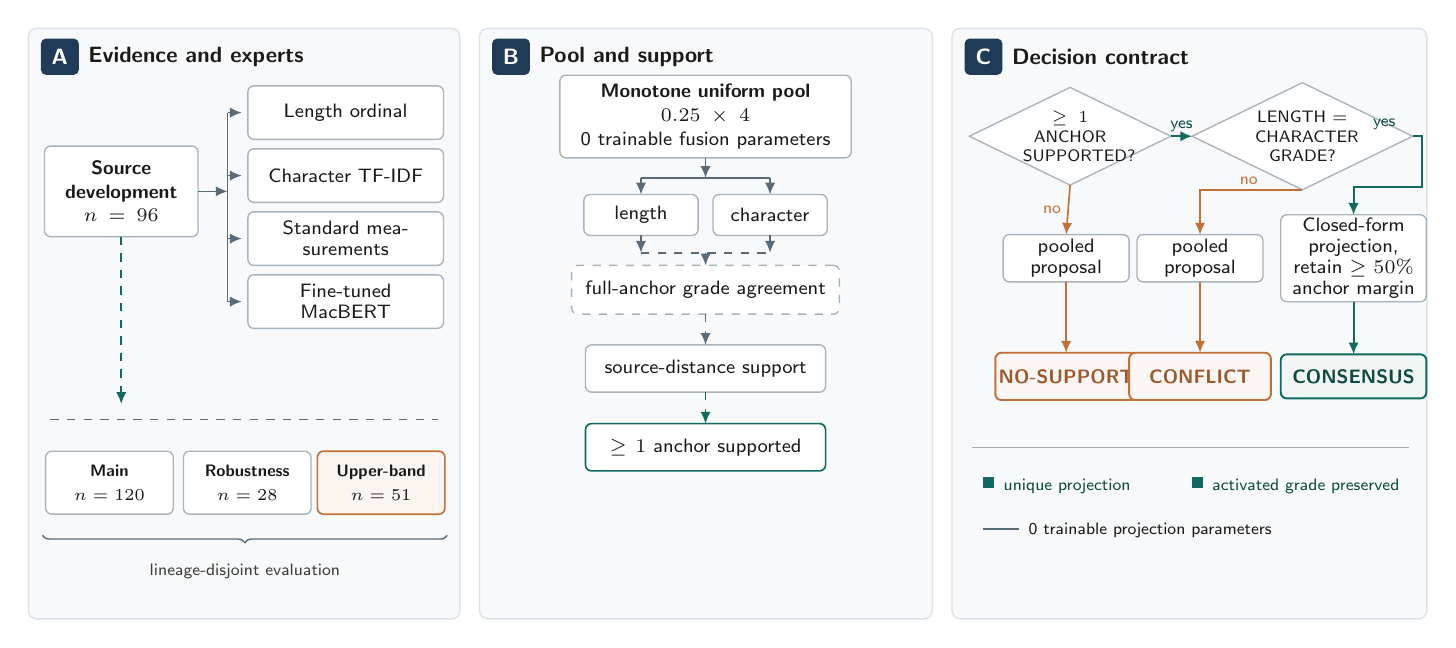
\begin{tikzpicture}[
  x=1cm, y=1cm,
  font=\sffamily,
  >={Latex[length=1.5mm,width=1.3mm]},
  every node/.style={inner sep=1.2pt, outer sep=0pt},
  panelbg/.style={draw=PANELB, line width=0.5pt, rounded corners=3pt, fill=PANELF},
  badge/.style={rounded corners=1.8pt, fill=NAVY, text=white,
                font=\sffamily\bfseries\fontsize{7.6}{7.6}\selectfont,
                minimum width=4.8mm, minimum height=4.6mm, inner sep=0pt},
  hdr/.style={font=\sffamily\bfseries\fontsize{7.8}{7.8}\selectfont,
              text=INK, anchor=west},
  flow/.style={draw=BORDER, line width=0.5pt, rounded corners=2.2pt, fill=white,
               align=center, font=\sffamily\fontsize{6.6}{7.6}\selectfont, text=INK},
  fam/.style={draw=BORDER, line width=0.5pt, rounded corners=2.2pt, fill=white,
              align=center, font=\sffamily\fontsize{6.6}{7.6}\selectfont, text=INK,
              text width=2.40cm, minimum height=6.8mm},
  coll/.style={draw=BORDER, line width=0.5pt, rounded corners=2.2pt, fill=white,
               align=center, font=\sffamily\fontsize{6.5}{7.5}\selectfont, text=INK,
               minimum width=1.62cm, minimum height=8.0mm},
  lock/.style={draw=WARN, line width=0.6pt, rounded corners=2.2pt, fill=WARN!7,
               align=center, font=\sffamily\fontsize{6.5}{7.5}\selectfont, text=INK,
               minimum width=1.62cm, minimum height=8.0mm},
  dectxt/.style={align=center, font=\sffamily\fontsize{6.2}{7.2}\selectfont,
                 text=INK, text width=1.20cm},
  cons/.style={draw=OK, line width=0.7pt, rounded corners=2.2pt, fill=OK!6,
               align=center, font=\sffamily\bfseries\fontsize{6.6}{7.6}\selectfont,
               text=OK!70!black},
  fail/.style={draw=WARN, line width=0.7pt, rounded corners=2.2pt, fill=WARN!6,
               align=center, font=\sffamily\bfseries\fontsize{6.6}{7.6}\selectfont,
               text=WARN!80!black},
  ar/.style={draw=LINE, line width=0.6pt, ->},
  ard/.style={draw=LINE, line width=0.6pt, ->, dashed},
  arok/.style={draw=OK, line width=0.7pt, ->},
  arno/.style={draw=WARN, line width=0.6pt, ->},
  lab/.style={font=\sffamily\fontsize{6.0}{7.0}\selectfont, text=INK},
  laby/.style={font=\sffamily\fontsize{6.0}{7.0}\selectfont, text=OK!70!black},
  labn/.style={font=\sffamily\fontsize{6.0}{7.0}\selectfont, text=WARN},
]

% ===================================================== panel backgrounds
\draw[panelbg] (0.12,2.12) rectangle (5.60,9.62);
\draw[panelbg] (5.85,2.12) rectangle (11.60,9.62);
\draw[panelbg] (11.85,2.12) rectangle (17.88,9.62);

% ============================================================ panel A
\node[badge] at (0.52,9.26) {A};
\node[hdr]  at (0.84,9.26) {Evidence and experts};

\node[fam, minimum width=1.95cm, minimum height=1.15cm, text width=1.72cm]
  (src) at (1.30,7.55) {\textbf{Source}\\[1pt]\textbf{development}\\[1pt]$n = 96$};

\foreach \yy/\t in {8.55/Length ordinal, 7.75/Character TF-IDF,
                    6.95/Standard measurements, 6.15/Fine-tuned MacBERT}{
  \node[fam] at (4.15,\yy) {\t};
}
\draw[ar] (src.east) -- (2.65,7.55);
\draw[LINE, line width=0.6pt] (2.65,6.15) -- (2.65,8.55);
\foreach \yy in {8.55,7.75,6.95,6.15}{ \draw[ar] (2.65,\yy) -- (2.83,\yy); }

\draw[ard, draw=OK] (src.south) -- (1.30,4.85);

\draw[LINE, line width=0.5pt, dashed] (0.40,4.65) -- (5.32,4.65);
\node[coll] (cmain) at (1.15,3.85) {\textbf{Main}\\[1pt]$n = 120$};
\node[coll] (crob)  at (2.90,3.85) {\textbf{Robustness}\\[1pt]$n = 28$};
\node[lock] (cub)   at (4.60,3.85) {\textbf{Upper-band}\\[1pt]$n = 51$};

\draw[decorate, decoration={brace, amplitude=2.6pt, mirror}, LINE, line width=0.5pt]
  (0.30,3.18) -- (5.44,3.18);
\node[lab, text=INK!85] at (2.87,2.72) {lineage-disjoint evaluation};

% ============================================================ panel B
\node[badge] at (6.25,9.26) {B};
\node[hdr]  at (6.57,9.26) {Pool and support};

\node[flow, minimum width=3.70cm, minimum height=1.05cm, text width=3.44cm]
  (pool) at (8.72,8.50) {\textbf{Monotone uniform pool}\\[1pt]$0.25 \times 4$\\[1pt]0 trainable fusion parameters};

\node[flow, minimum width=1.45cm, minimum height=0.52cm] (len) at (7.90,7.25) {length};
\node[flow, minimum width=1.45cm, minimum height=0.52cm] (chr) at (9.54,7.25) {character};
\draw[ar] (pool.south) -- (8.72,7.72);
\draw[LINE, line width=0.6pt] (7.90,7.72) -- (9.54,7.72);
\draw[ar] (7.90,7.72) -- (len.north);
\draw[ar] (9.54,7.72) -- (chr.north);

\node[flow, dashed, minimum width=3.40cm, minimum height=0.62cm, text width=3.16cm]
  (agree) at (8.72,6.30) {full-anchor grade agreement};
\draw[LINE, line width=0.6pt, dashed] (7.90,6.77) -- (9.54,6.77);
\draw[ard] (len.south) -- (7.90,6.77);
\draw[ard] (chr.south) -- (9.54,6.77);
\draw[ard] (8.72,6.77) -- (agree.north);

\node[flow, minimum width=3.05cm, minimum height=0.60cm, text width=2.83cm]
  (supp) at (8.72,5.30) {source-distance support};
\draw[ard] (agree.south) -- (supp.north);

\node[flow, draw=OK, line width=0.6pt, minimum width=3.05cm, minimum height=0.60cm,
      text width=2.83cm] (anch) at (8.72,4.30) {$\geq 1$ anchor supported};
\draw[ard, draw=OK] (supp.south) -- (anch.north);

% ============================================================ panel C
\node[badge] at (12.25,9.26) {C};
\node[hdr]  at (12.57,9.26) {Decision contract};

% decision nodes as explicit polygons (predictable inscribed area)
\draw[BORDER, fill=white, line width=0.5pt]
  (12.07,8.25) -- (13.35,8.87) -- (14.63,8.25) -- (13.35,7.63) -- cycle;
\node[dectxt] at (13.35,8.25) {$\geq 1$ ANCHOR\\SUPPORTED?};

\draw[BORDER, fill=white, line width=0.5pt]
  (14.90,8.25) -- (16.30,8.93) -- (17.70,8.25) -- (16.30,7.57) -- cycle;
\node[dectxt] at (16.30,8.25) {LENGTH $=$\\CHARACTER\\GRADE?};

\draw[arok] (14.63,8.25) -- node[laby, above, yshift=0.4pt]{yes} (14.90,8.25);

\node[flow, minimum width=1.85cm, minimum height=1.10cm, text width=1.63cm]
  (proj) at (16.95,6.70) {Closed-form projection, retain $\geq 50\%$ anchor margin};
\draw[arok] (17.70,8.25) -- (17.82,8.25) -- (17.82,7.60) -- (16.95,7.60) -- (proj.north);
\node[laby] at (17.34,8.40) {yes};

\node[cons, minimum width=1.85cm, minimum height=0.56cm] (consbox) at (16.95,5.20) {CONSENSUS};
\draw[arok] (proj.south) -- (consbox.north);

\node[flow, minimum width=1.60cm, minimum height=0.60cm] (pp1) at (13.30,6.70) {pooled\\proposal};
\draw[arno] (13.35,7.63) -- node[labn, left, xshift=-1.4pt]{no} (pp1.north);
\node[fail, minimum width=1.80cm, minimum height=0.60cm] (nosup) at (13.30,5.20) {NO-SUPPORT};
\draw[arno] (pp1.south) -- (nosup.north);

\node[flow, minimum width=1.60cm, minimum height=0.60cm] (pp2) at (15.00,6.70) {pooled\\proposal};
\draw[arno] (16.30,7.57) -- (15.00,7.57) -- (pp2.north);
\node[labn] at (15.62,7.68) {no};
\node[fail, minimum width=1.80cm, minimum height=0.60cm] (conf) at (15.00,5.20) {CONFLICT};
\draw[arno] (pp2.south) -- (conf.north);

% legend, returned to the panel now that the type is large enough to read
\draw[LINE!55, line width=0.5pt] (12.10,4.30) -- (17.66,4.30);
\node[lab, anchor=west, text=OK!70!black] at (12.20,3.82)
  {\textcolor{OK}{\rule[1.0pt]{4.0pt}{4.0pt}}\;\;unique projection};
\node[lab, anchor=west, text=OK!70!black] at (14.85,3.82)
  {\textcolor{OK}{\rule[1.0pt]{4.0pt}{4.0pt}}\;\;activated grade preserved};
\node[lab, anchor=west] at (12.20,3.24)
  {\textcolor{LINE}{\rule[1.6pt]{13pt}{0.8pt}}\;\;0 trainable projection parameters};
\end{tikzpicture}
}
\caption{RA-SCOPE dataflow. Four monotone experts form a parameter-free uniform
pool. The decision contract first checks whether at least one anchor is
source-supported, then whether the length and character grades agree. Supported
agreement activates projection and returns CONSENSUS; supported disagreement
retains the pool and returns CONFLICT; absence of support retains the pool and
returns NO-SUPPORT.}
\label{fig:dataflow}
\end{figure*}

%=====================================================================
\section{Experimental Protocol}
%=====================================================================

\noindent\textbf{Comparators.} We report each expert and the unprojected uniform
pool. A contemporary prompt baseline uses Qwen2.5-3B-Instruct~\cite{qwen2024technical}:
a fixed Chinese six-level rubric, the full extracted book text, and restricted
next-token scoring over the six level tokens. It has no demonstrations,
generation sampling, or target-label selection. Projection ablations require
both anchors to be supported, activate on an agreeing qualified subset, or
remove the support condition while retaining full agreement.

\noindent\textbf{Metrics and uncertainty.} The primary metric is quadratic
weighted kappa (QWK)~\cite{cohen1968weighted}. We also report MAE, exact
accuracy, within-one accuracy, and errors above one level. Probability
diagnostics comprise threshold-averaged ordinal Brier score, class negative
log-likelihood (NLL), 10-bin expected calibration error (ECE), and MAE
risk--coverage area (RC-AUC); lower is better. All method differences use
10{,}000 paired percentile-bootstrap samples over original-work
lineages~\cite{efron1993introduction}. Support cutoffs
$u \in \{.50,.60,.70,.80,.90,.95\}$ and margin relaxations in $\{.25,.50,.75\}$
test sensitivity.

\noindent\textbf{Reproducibility.} The PyTorch module consumes raw cumulative
probabilities and exposes every support state. Tests cover monotonicity,
full-consensus activation, single-supported-anchor disagreement, unsupported
agreement, preservation, invalid inputs, and zero trainable parameters. The
artifact records source folds, per-book predictions, bootstrap outputs, exact
model identifiers, prompt hashes, and SHA-256 inventories.

%=====================================================================
\section{Results}
%=====================================================================

\subsection{Global Grading}
RA-SCOPE reaches .823 QWK and .417 MAE on the main collection
(Table~\ref{tab:main}). Two properties matter more for deployment than the
QWK delta. First, the rate of errors exceeding one level falls from .017 for the
uniform pool to .008, halving a failure mode that is far costlier than an
off-by-one grade. Second, the gains over the strongest individual comparator are
substantial and their intervals are far from zero: $+.060$ $[.008,.118]$ QWK and
$-{.142}$ $[-.250,-.033]$ MAE against fine-tuned MacBERT, and $+.285$
$[.173,.403]$ QWK and $-.408$ $[-.600,-.217]$ MAE against the Qwen2.5-3B rubric
baseline. Relative to uniform pooling---itself a strong heterogeneous
baseline---the direct QWK gain is $+.032$ $[.005,.066]$ with an MAE change of
$-.042$ $[-.092,.008]$.

Source-only out-of-fold predictions obtain .858 QWK and .406 MAE with one error
above one level among 96 books. On the separate robustness collection
RA-SCOPE obtains .786 QWK, .393 MAE, 60.7\% exact accuracy and 100\% within one
level; its gains over MacBERT and Qwen are $+.114$ $[.030,.227]$ and $+.183$
$[.008,.313]$ QWK respectively. The interval against length includes zero, as
expected for 28 books.

\begin{table}[t]
\caption{Global Grading. Ablations change only projection activation.}
\label{tab:main}
\centering
\footnotesize
\setlength{\tabcolsep}{3.2pt}
\begin{tabular}{lcccccc}
\toprule
& \multicolumn{4}{c}{Main ($n{=}120$)} & \multicolumn{2}{c}{Rob. ($n{=}28$)} \\
\cmidrule(lr){2-5}\cmidrule(lr){6-7}
Method & QWK & MAE & Exact & $>\!1$ & QWK & MAE \\
\midrule
Character TF--IDF      & .577 & .708 & .425 & .125 & .487 & .786 \\
Length ordinal         & .767 & .542 & .492 & .025 & .772 & .429 \\
Standard measurements  & .622 & .633 & .467 & .083 & .620 & .536 \\
MacBERT (3 seeds)      & .763 & .558 & .467 & .025 & .672 & .571 \\
Qwen2.5-3B rubric      & .538 & .825 & .425 & .183 & .603 & .714 \\
Uniform probability pool & .790 & .458 & .558 & .017 & .786 & .393 \\
\midrule
RA-SCOPE               & \textbf{.823} & \textbf{.417} & \textbf{.592} & \textbf{.008} & \textbf{.786} & \textbf{.393} \\
\bottomrule
\end{tabular}
\end{table}

\subsection{What the Support Contract Guarantees}
The support contract is a decision-audit mechanism rather than an accuracy
lever. On these collections the three unsupported agreements do not cross a
decision threshold, so disabling the support condition yields identical point
grades (Table~\ref{tab:states}); requiring both anchors to be supported gives
.815/.425 and allowing a singleton qualified subset to activate gives .799/.450.
The contract's value appears instead in the state distribution it exposes. The
main collection contains 38 support-backed full consensuses, 46 supported
conflicts, and 36 books without a supported anchor, with exact accuracy .711,
.565 and .500 respectively. The state is therefore informative even though
every route returns a prediction, and it is exact rather than fitted: the
projection preserves 38/38 activated grades on the main collection, 32/32 on
source out-of-fold predictions, and 7/7 on the robustness collection. Across
support cutoffs, main QWK stays in $[.817,.825]$, and every tested retained
margin produces identical point grades.

\begin{table}[t]
\caption{Support States on the Main Collection. Every route returns a grade.}
\label{tab:states}
\centering
\footnotesize
\begin{tabular}{lccp{3.3cm}}
\toprule
State & $n$ & Exact & Route \\
\midrule
CONSENSUS  & 38 & .711 & Projection applied; grade preserved \\
CONFLICT   & 46 & .565 & Pooled proposal retained \\
NO-SUPPORT & 36 & .500 & Pooled proposal retained \\
\bottomrule
\end{tabular}
\end{table}

\begin{figure*}[!t]
\centering
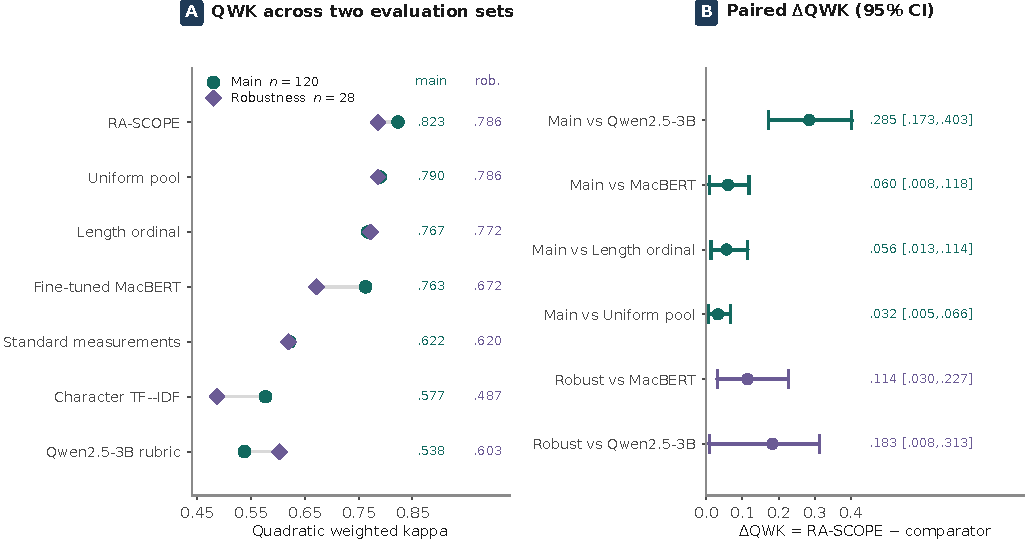
\includegraphics[width=\textwidth]{fig2_performance.pdf}
\caption{Primary ordinal performance. (a)~Main and robustness QWK across
RA-SCOPE and six comparators; circles and diamonds distinguish the two
independently adjudicated collections. (b)~Direct paired QWK gains for the four
prespecified main comparisons and two robustness comparisons; bars are 95\%
lineage-bootstrap intervals.}
\label{fig:performance}
\end{figure*}

\subsection{Learned Fusion Baseline}
\label{sec:stack}
RA-SCOPE is deliberately zero-parameter, so the natural objection is that a
fitted fusion over the same experts would do better. As a post-hoc analysis we
test this directly.
Using the four experts' continuous ordinal scores from the frozen artifact we
fit a multinomial logistic regression on the 120-book collection under
stratified $k$-fold cross-validation ($k\in\{4,5,6,10\}$, ten seeds each) and
pool the out-of-fold predictions; Table~\ref{tab:stack} reports the $k{=}5$
result. Learned fusion is competitive on QWK and clearly better on absolute
error. Its QWK is .844 against .823 (difference $+.025$, 95\% book-bootstrap CI
$[-.023,+.074]$, i.e.\ not distinguishable at this sample size), but its MAE is
.275 against .417 (difference $-.142$, CI $[-.250,-.042]$) and its
catastrophic-error rate is .002 against .008. Per book, the stacked model has
lower absolute error on 30 items, the same on 77 and higher on 13, and the
result is stable across all four fold counts.

The comparison is not a like-for-like substitution, and the difference is
precisely the property RA-SCOPE was designed for. The stacked model is fitted
with access to target-collection labels: it cannot be constructed for a
platform on which no adjudicated books exist, and its per-item decision rule is
a fitted weight vector rather than an inspectable contract. RA-SCOPE consumes no
target labels and every activated consensus grade remains provably preserved.
We therefore read Table~\ref{tab:stack} as the measured price of auditability on
this collection rather than as a defect of the contract: on MAE the contract
pays about .14 levels while retaining the guarantee, the state semantics and
cold-start operation.

\begin{table}[t]
\caption{Learned Fusion Versus the Zero-Parameter Contract. The stacked row is
the mean over ten seeds at $k{=}5$; intervals are given in the text.}
\label{tab:stack}
\centering
\footnotesize
\setlength{\tabcolsep}{5pt}
\begin{tabular}{lcccc}
\toprule
Method & QWK & MAE & Exact & $>\!1$ \\
\midrule
RA-SCOPE (no target labels)      & .823 & .417 & .592 & .008 \\
Stacked logistic (5-fold CV)     & \textbf{.844} & \textbf{.275} & \textbf{.727} & \textbf{.002} \\
\midrule
Difference                       & $+.025$ & $-.142$ & $+.135$ & $-.006$ \\
\bottomrule
\end{tabular}
\end{table}

\subsection{Expert Complementarity and Probability Quality}
The ensemble is not averaging replicas. Its four experts disagree on 104/120
main books, with mean pairwise disagreement .576 and 42 distinct prediction
patterns. Each expert is uniquely exact on at least four books (length 4,
character 12, measurements 10, MacBERT 6), and at least one expert is exact on
85.8\% of books. RA-SCOPE is exact on 60 disagreement cases, four more than
uniform pooling, including one book on which no individual point prediction is
exact. The robustness set shows a similar mean pairwise disagreement of .589.

Point accuracy and probability quality separate cleanly. Projection improves
the uniform pool's Brier score (.085 to .083), NLL (1.443 to 1.411) and
selective RC-AUC (.437 to .418), with a small ECE trade-off (.187 to .203).
Length has the best Brier/NLL (.080/1.306) but substantially worse ECE (.274)
and selective risk (.543), and Qwen has the weakest values on all four
(.129/2.020/.269/.749). The QWK gains therefore do not come from globally
sharpening probabilities without regard to ranking or coverage.

\subsection{Length, Source, and Level Stress Tests}
RA-SCOPE's continuous score has Spearman $\rho = .901$ with the gold level.
After residualising both variables for log character count, log page count and
source, partial $\rho = .400$ $[.258,.545]$, whereas the length expert gives
$-.034$ $[-.091,.090]$; their paired partial-correlation difference is
$[.238,.573]$. On 24 disjoint counter-length pairs---where character count
orders two books opposite to their gold levels---RA-SCOPE orders the pair
correctly with .708 accuracy $[.500,.875]$, compared with .000 for length by
construction. On 56 nearest different-level disjoint pairs it reaches .875
$[.786,.946]$. Source slices are consistent with the aggregate result:
StoryWeaver ($n{=}89$) yields .775 QWK/.416 MAE and Global ASP ($n{=}23$)
.795/.391; the eight-book GDL slice is descriptive (.543/.500). Band-wise MAE
is .500 for L1--L2, .375 for L3 and .353 for L4--L5, below length and MacBERT
in every band.

\begin{figure*}[!t]
\centering
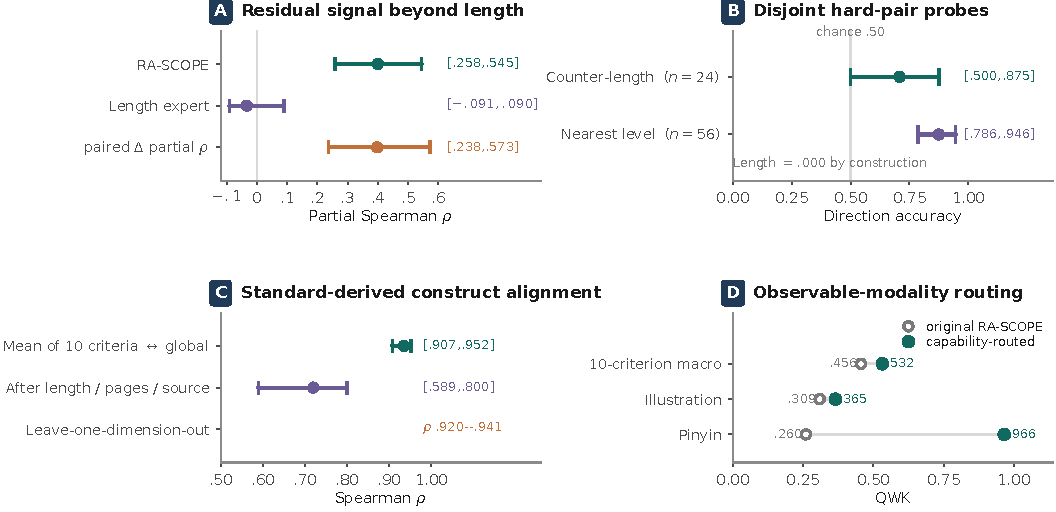
\includegraphics[width=\textwidth]{fig3_validity.pdf}
\caption{Validity beyond aggregate accuracy. (a)~Partial Spearman correlations
after controlling length, page count and source. (b)~Direction accuracy on
disjoint counter-length and nearest different-level pairs. (c)~Convergent
alignment between the global grade and Standard-derived criteria.
(d)~Criterion-level gains from routing illustration and pinyin to
observable-modality specialists.}
\label{fig:validity}
\end{figure*}

\subsection{Construct and Modality Evidence}
The mean of the ten adjudicated criterion grades correlates .935
$[.907,.952]$ with the global grade. Controlling log characters, log pages and
source leaves partial $\rho = .720$ $[.589,.800]$, and leaving out any single
criterion keeps the raw correlation between .920 and .941. This convergent
evidence links the global target to the Standard's operational dimensions
rather than to length alone. For criterion prediction, observable-modality
specialists improve macro-QWK from .456 to .532, a paired gain of .076
$[.055,.096]$, and reduce macro-MAE by .119 $[-.158,-.082]$. DINOv2
illustration features~\cite{oquab2024dinov2} improve illustration-independence
QWK from .309 to .365 and MAE from 1.092 to .925; deterministic pinyin features
improve QWK from .260 to .966 and MAE from 1.125 to .100. Layout remains on the
text route because source families expose incomparable page geometry.

%=====================================================================
\section{Deployment and Human-in-the-Loop Review}
\label{sec:deploy}
%=====================================================================

RA-SCOPE is designed to sit inside an existing review process rather than to
replace it, and the measurements above translate directly into operating
behaviour.

\noindent\textbf{Cost.} The layer itself is closed-form and adds negligible
overhead to the four experts it composes. The expensive components are the
experts: MacBERT training used one RTX~4060 Laptop GPU for approximately 7.7
GPU-minutes across three seeds, and the Qwen2.5-3B rubric baseline scored 244
books in 237~seconds using bfloat16 with 8.93~GB peak allocated GPU memory. The
pooled projection is a coordinate-wise clip (Eq.~\ref{eq:clip}) and can be
re-executed by a reviewer by hand.

\noindent\textbf{Triage.} Because exact accuracy stratifies by state
(.711/.565/.500), a workflow can auto-accept CONSENSUS items and route CONFLICT
and NO-SUPPORT items to human adjudication. On the main collection this
concentrates scarce expert time on 82 of 120 books while the 38 automatically
accepted items are the ones on which the system is most accurate. Nothing is
hidden: every item still receives an ordinal distribution, and the state is
reported alongside it.

\noindent\textbf{Preservation.} The guarantee in Proposition~2 is what makes
auto-acceptance defensible. When the two anchors agree and at least one is
support-eligible, the projection provably returns that agreed grade---observed
as 38/38, 32/32 and 7/7 preservation on the main, source out-of-fold and
robustness collections. Adopting a CONSENSUS grade therefore cannot overturn a
decision that the evidence already supported.

\noindent\textbf{Cold start on a new platform.} Fitting the experts and
calibrating the support rank requires only the 96-book source-development
collection; no labels from the new platform are needed. This is where the
zero-parameter design pays for itself, because the stacked fusion of
Section~\ref{sec:stack} cannot be constructed at all until adjudicated books
exist on the target platform. Source-slice results
(.775 QWK for StoryWeaver, .795 for Global ASP) indicate that the same
configuration transfers across platforms, and the per-item support state makes
any residual misfit visible instead of silent.

%=====================================================================
\section{Discussion}
%=====================================================================

RA-SCOPE separates three questions that ordinary fusion merges: what the
experts propose, whether anchor evidence resembles the source, and which
decisions the ensemble is allowed to alter. The support rank is label-free;
full agreement prevents a singleton from masquerading as consensus; and the
convex projection turns the decision rule into a unique, executable operation.
These properties make the guarantee inspectable per book while retaining a
complete ordinal distribution.

The empirical pattern is equally specific. Uniform pooling already supplies a
strong heterogeneous baseline. Projection changes only nine main-set absolute
errors relative to that pool (seven improve, two worsen), yet this is enough for
a positive paired QWK interval and halves the frequency of errors above one
level. Gains over length survive covariate control and counter-length
comparisons, while the Qwen rubric baseline reveals substantial platform
sensitivity despite explicit instructions not to use length alone. Capability
routing further shows that illustration and pinyin criteria benefit from
evidence unavailable to a text-only global model.

\noindent\textbf{Why zero-parameter pooling rather than learned fusion.}
Zero-parameter pooling is a design requirement, not a convenience. A learned
fusion layer must be fitted on labelled books; because source platforms differ
sharply in layout, length and illustration conventions, such a layer transfers
its fitting-platform label distribution to new platforms, and its per-item
weights are not inspectable. RA-SCOPE consumes exactly one quantity from
held-out data---a label-free distance rank---so Eq.~\ref{eq:clip} can be
re-executed and audited item by item. Where a fitted alternative is affordable
it does raise average fit: the stacked fusion of Section~\ref{sec:stack} reduces
MAE by .142 relative to the contract. Our claim concerns decision guarantees and
auditability under platform shift, not the best average fit on a labelled target
collection.

%=====================================================================
\section{Limitations and Ethical Considerations}
%=====================================================================

Observed gold labels contain four L5 books and no L6 books, and the 28-book
robustness collection is small; the results therefore support L1--L4 use most
directly, with L5 descriptive and L6 untested. Material grades are not
learner-comprehension outcomes. Architecture selection had access to the
adjudicated collections, so a prospectively untouched, upper-level sample
remains necessary for deployment-level validation. The conformal interpretation
of the support rank requires exchangeable calibration and target
representations, and platform shift can violate that assumption; a high support
rank does not imply prediction correctness, and two supported anchors can share
an error. StoryWeaver dominates the main collection, while the smallest source
slice has eight books. The Qwen experiment is a reproducible 3B zero-shot
rubric baseline, not a claim about all larger or proprietary LLMs. OCR, page
extraction and DINOv2 style sensitivity can introduce source-specific error,
and comparable geometric evidence is still needed for a dedicated layout
specialist.

The study uses books and adult professional annotations, with no learner records
or children's personal data. Annotators are represented by role identifiers,
and independent ratings precede separate adjudication. Predictions are intended
to assist human material review: conflict, no-support and upper-band cases
remain visible rather than being presented as certified decisions. Restricted
book text and illustrations remain with their source providers, and users must
preserve applicable attribution and licence conditions. The Standard may
privilege standard written Mandarin and conventional print layouts; dialectal,
culturally specific, accessibility-relevant and visually driven materials
require human validation.

%=====================================================================
\section{Conclusion}
%=====================================================================

We presented a support-backed full-consensus projection for ordinal picturebook
grading. It combines four monotone experts without fitted fusion parameters,
attaches an explicit support state to every item, and uniquely preserves every
activated anchor-consensus grade. Across source-only out-of-fold, main and
separate robustness evaluations it improves the strongest individual experts
and the uniform pool while remaining stable across support and margin settings.
The result is a compact inference architecture whose accuracy, decision
semantics and evidence boundary can all be audited, and whose states translate
directly into human review triage.

%=====================================================================
\section*{Acknowledgment}
%=====================================================================

This work was supported by the National College Students' Innovation and
Entrepreneurship Training Program (No.~202610032033). The public artifact URL
will be added here before the camera-ready submission.

\bibliographystyle{IEEEtran}
\bibliography{refs}

\end{document}
